% Created by tikzDevice version 0.11 on 2018-04-15 12:26:52
% !TEX encoding = UTF-8 Unicode
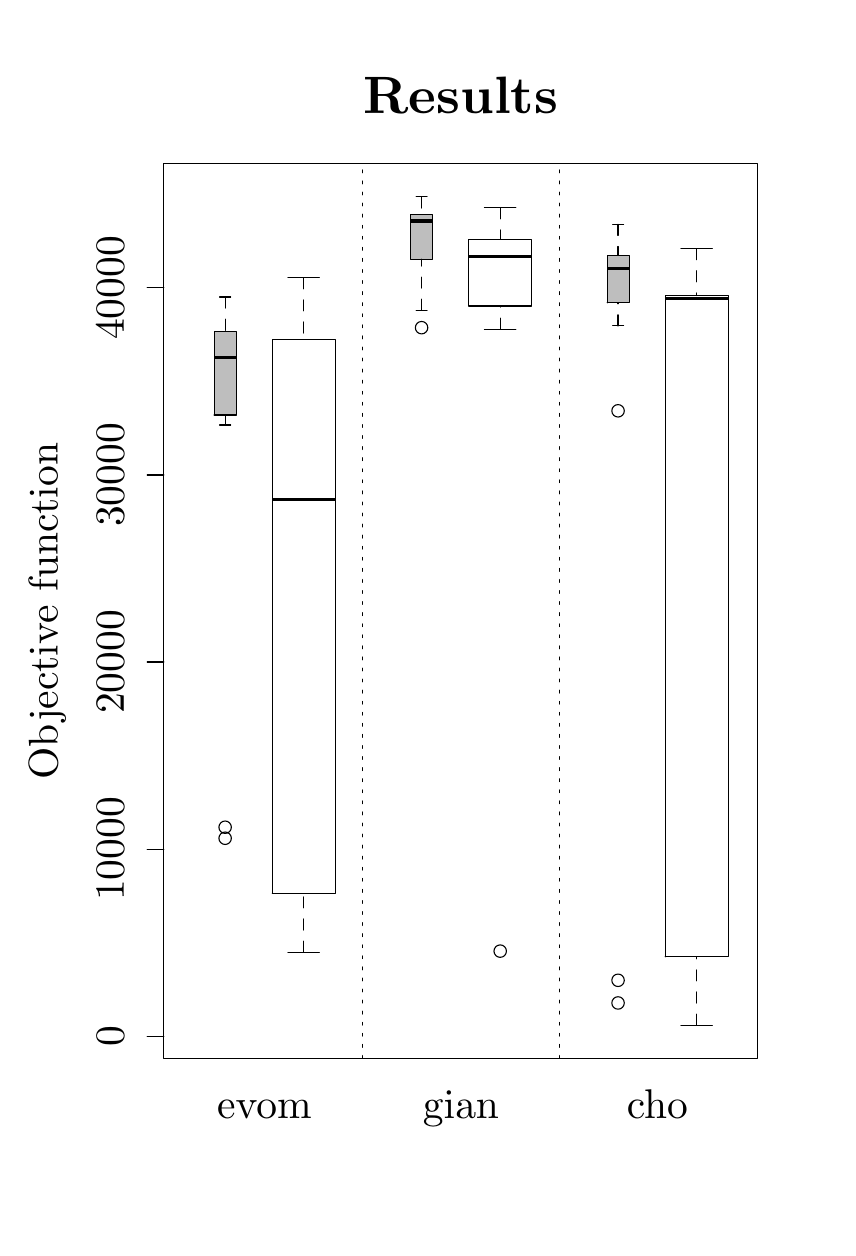
\begin{tikzpicture}[x=1pt,y=1pt]
\definecolor{fillColor}{RGB}{255,255,255}
\path[use as bounding box,fill=fillColor,fill opacity=0.00] (0,0) rectangle (289.08,433.62);
\begin{scope}
\path[clip] ( 49.20, 61.20) rectangle (263.88,384.42);
\definecolor{fillColor}{RGB}{190,190,190}

\path[fill=fillColor] ( 67.37,293.66) --
	( 75.33,293.66) --
	( 75.33,323.85) --
	( 67.37,323.85) --
	cycle;
\definecolor{drawColor}{RGB}{0,0,0}

\path[draw=drawColor,line width= 1.2pt,line join=round] ( 67.37,314.32) -- ( 75.33,314.32);

\path[draw=drawColor,line width= 0.4pt,dash pattern=on 4pt off 4pt ,line join=round,line cap=round] ( 71.35,290.03) -- ( 71.35,293.66);

\path[draw=drawColor,line width= 0.4pt,dash pattern=on 4pt off 4pt ,line join=round,line cap=round] ( 71.35,336.28) -- ( 71.35,323.85);

\path[draw=drawColor,line width= 0.4pt,line join=round,line cap=round] ( 69.36,290.03) -- ( 73.34,290.03);

\path[draw=drawColor,line width= 0.4pt,line join=round,line cap=round] ( 69.36,336.28) -- ( 73.34,336.28);

\path[draw=drawColor,line width= 0.4pt,line join=round,line cap=round] ( 67.37,293.66) --
	( 75.33,293.66) --
	( 75.33,323.85) --
	( 67.37,323.85) --
	( 67.37,293.66);

\path[draw=drawColor,line width= 0.4pt,line join=round,line cap=round] ( 71.35,140.72) circle (  2.25);

\path[draw=drawColor,line width= 0.4pt,line join=round,line cap=round] ( 71.35,144.70) circle (  2.25);
\definecolor{fillColor}{RGB}{255,255,255}

\path[fill=fillColor] ( 88.39,120.78) --
	(111.11,120.78) --
	(111.11,321.02) --
	( 88.39,321.02) --
	cycle;

\path[draw=drawColor,line width= 1.2pt,line join=round] ( 88.39,263.10) -- (111.11,263.10);

\path[draw=drawColor,line width= 0.4pt,dash pattern=on 4pt off 4pt ,line join=round,line cap=round] ( 99.75, 99.55) -- ( 99.75,120.78);

\path[draw=drawColor,line width= 0.4pt,dash pattern=on 4pt off 4pt ,line join=round,line cap=round] ( 99.75,343.28) -- ( 99.75,321.02);

\path[draw=drawColor,line width= 0.4pt,line join=round,line cap=round] ( 94.07, 99.55) -- (105.43, 99.55);

\path[draw=drawColor,line width= 0.4pt,line join=round,line cap=round] ( 94.07,343.28) -- (105.43,343.28);

\path[draw=drawColor,line width= 0.4pt,line join=round,line cap=round] ( 88.39,120.78) --
	(111.11,120.78) --
	(111.11,321.02) --
	( 88.39,321.02) --
	( 88.39,120.78);
\definecolor{fillColor}{RGB}{190,190,190}

\path[fill=fillColor] (138.37,349.96) --
	(146.32,349.96) --
	(146.32,365.98) --
	(138.37,365.98) --
	cycle;

\path[draw=drawColor,line width= 1.2pt,line join=round] (138.37,363.76) -- (146.32,363.76);

\path[draw=drawColor,line width= 0.4pt,dash pattern=on 4pt off 4pt ,line join=round,line cap=round] (142.34,331.50) -- (142.34,349.96);

\path[draw=drawColor,line width= 0.4pt,dash pattern=on 4pt off 4pt ,line join=round,line cap=round] (142.34,372.45) -- (142.34,365.98);

\path[draw=drawColor,line width= 0.4pt,line join=round,line cap=round] (140.35,331.50) -- (144.33,331.50);

\path[draw=drawColor,line width= 0.4pt,line join=round,line cap=round] (140.35,372.45) -- (144.33,372.45);

\path[draw=drawColor,line width= 0.4pt,line join=round,line cap=round] (138.37,349.96) --
	(146.32,349.96) --
	(146.32,365.98) --
	(138.37,365.98) --
	(138.37,349.96);

\path[draw=drawColor,line width= 0.4pt,line join=round,line cap=round] (142.34,325.21) circle (  2.25);
\definecolor{fillColor}{RGB}{255,255,255}

\path[fill=fillColor] (159.38,333.03) --
	(182.10,333.03) --
	(182.10,357.23) --
	(159.38,357.23) --
	cycle;

\path[draw=drawColor,line width= 1.2pt,line join=round] (159.38,350.89) -- (182.10,350.89);

\path[draw=drawColor,line width= 0.4pt,dash pattern=on 4pt off 4pt ,line join=round,line cap=round] (170.74,324.65) -- (170.74,333.03);

\path[draw=drawColor,line width= 0.4pt,dash pattern=on 4pt off 4pt ,line join=round,line cap=round] (170.74,368.52) -- (170.74,357.23);

\path[draw=drawColor,line width= 0.4pt,line join=round,line cap=round] (165.06,324.65) -- (176.42,324.65);

\path[draw=drawColor,line width= 0.4pt,line join=round,line cap=round] (165.06,368.52) -- (176.42,368.52);

\path[draw=drawColor,line width= 0.4pt,line join=round,line cap=round] (159.38,333.03) --
	(182.10,333.03) --
	(182.10,357.23) --
	(159.38,357.23) --
	(159.38,333.03);

\path[draw=drawColor,line width= 0.4pt,line join=round,line cap=round] (170.74, 99.93) circle (  2.25);
\definecolor{fillColor}{RGB}{190,190,190}

\path[fill=fillColor] (209.36,334.20) --
	(217.31,334.20) --
	(217.31,351.31) --
	(209.36,351.31) --
	cycle;

\path[draw=drawColor,line width= 1.2pt,line join=round] (209.36,346.60) -- (217.31,346.60);

\path[draw=drawColor,line width= 0.4pt,dash pattern=on 4pt off 4pt ,line join=round,line cap=round] (213.33,325.84) -- (213.33,334.20);

\path[draw=drawColor,line width= 0.4pt,dash pattern=on 4pt off 4pt ,line join=round,line cap=round] (213.33,362.55) -- (213.33,351.31);

\path[draw=drawColor,line width= 0.4pt,line join=round,line cap=round] (211.35,325.84) -- (215.32,325.84);

\path[draw=drawColor,line width= 0.4pt,line join=round,line cap=round] (211.35,362.55) -- (215.32,362.55);

\path[draw=drawColor,line width= 0.4pt,line join=round,line cap=round] (209.36,334.20) --
	(217.31,334.20) --
	(217.31,351.31) --
	(209.36,351.31) --
	(209.36,334.20);

\path[draw=drawColor,line width= 0.4pt,line join=round,line cap=round] (213.33,295.17) circle (  2.25);

\path[draw=drawColor,line width= 0.4pt,line join=round,line cap=round] (213.33, 81.20) circle (  2.25);

\path[draw=drawColor,line width= 0.4pt,line join=round,line cap=round] (213.33, 89.39) circle (  2.25);
\definecolor{fillColor}{RGB}{255,255,255}

\path[fill=fillColor] (230.37, 97.85) --
	(253.09, 97.85) --
	(253.09,336.79) --
	(230.37,336.79) --
	cycle;

\path[draw=drawColor,line width= 1.2pt,line join=round] (230.37,335.78) -- (253.09,335.78);

\path[draw=drawColor,line width= 0.4pt,dash pattern=on 4pt off 4pt ,line join=round,line cap=round] (241.73, 73.17) -- (241.73, 97.85);

\path[draw=drawColor,line width= 0.4pt,dash pattern=on 4pt off 4pt ,line join=round,line cap=round] (241.73,353.77) -- (241.73,336.79);

\path[draw=drawColor,line width= 0.4pt,line join=round,line cap=round] (236.05, 73.17) -- (247.41, 73.17);

\path[draw=drawColor,line width= 0.4pt,line join=round,line cap=round] (236.05,353.77) -- (247.41,353.77);

\path[draw=drawColor,line width= 0.4pt,line join=round,line cap=round] (230.37, 97.85) --
	(253.09, 97.85) --
	(253.09,336.79) --
	(230.37,336.79) --
	(230.37, 97.85);
\end{scope}
\begin{scope}
\path[clip] (  0.00,  0.00) rectangle (289.08,433.62);
\definecolor{drawColor}{RGB}{0,0,0}

\node[text=drawColor,rotate= 90.00,anchor=base,inner sep=0pt, outer sep=0pt, scale=  1.50] at ( 10.80,222.81) {Objective function};
\end{scope}
\begin{scope}
\path[clip] ( 49.20, 61.20) rectangle (263.88,384.42);
\definecolor{drawColor}{RGB}{0,0,0}

\path[draw=drawColor,line width= 0.4pt,dash pattern=on 1pt off 3pt ,line join=round,line cap=round] (121.04, 61.20) -- (121.04,384.42);

\path[draw=drawColor,line width= 0.4pt,dash pattern=on 1pt off 3pt ,line join=round,line cap=round] (192.04, 61.20) -- (192.04,384.42);
\end{scope}
\begin{scope}
\path[clip] (  0.00,  0.00) rectangle (289.08,433.62);
\definecolor{drawColor}{RGB}{0,0,0}

\node[text=drawColor,anchor=base,inner sep=0pt, outer sep=0pt, scale=  1.50] at ( 85.55, 39.60) {evom};

\node[text=drawColor,anchor=base,inner sep=0pt, outer sep=0pt, scale=  1.50] at (156.54, 39.60) {gian};

\node[text=drawColor,anchor=base,inner sep=0pt, outer sep=0pt, scale=  1.50] at (227.53, 39.60) {cho};
\end{scope}
\begin{scope}
\path[clip] (  0.00,  0.00) rectangle (289.08,433.62);
\definecolor{drawColor}{RGB}{0,0,0}

\node[text=drawColor,anchor=base,inner sep=0pt, outer sep=0pt, scale=  1.90] at (156.54,402.46) {\bfseries Results};
\end{scope}
\begin{scope}
\path[clip] (  0.00,  0.00) rectangle (289.08,433.62);
\definecolor{drawColor}{RGB}{0,0,0}

\path[draw=drawColor,line width= 0.4pt,line join=round,line cap=round] ( 49.20, 69.22) -- ( 49.20,339.57);

\path[draw=drawColor,line width= 0.4pt,line join=round,line cap=round] ( 49.20, 69.22) -- ( 43.20, 69.22);

\path[draw=drawColor,line width= 0.4pt,line join=round,line cap=round] ( 49.20,136.81) -- ( 43.20,136.81);

\path[draw=drawColor,line width= 0.4pt,line join=round,line cap=round] ( 49.20,204.40) -- ( 43.20,204.40);

\path[draw=drawColor,line width= 0.4pt,line join=round,line cap=round] ( 49.20,271.99) -- ( 43.20,271.99);

\path[draw=drawColor,line width= 0.4pt,line join=round,line cap=round] ( 49.20,339.57) -- ( 43.20,339.57);

\node[text=drawColor,rotate= 90.00,anchor=base,inner sep=0pt, outer sep=0pt, scale=  1.50] at ( 34.80, 69.22) {0};

\node[text=drawColor,rotate= 90.00,anchor=base,inner sep=0pt, outer sep=0pt, scale=  1.50] at ( 34.80,136.81) {10000};

\node[text=drawColor,rotate= 90.00,anchor=base,inner sep=0pt, outer sep=0pt, scale=  1.50] at ( 34.80,204.40) {20000};

\node[text=drawColor,rotate= 90.00,anchor=base,inner sep=0pt, outer sep=0pt, scale=  1.50] at ( 34.80,271.99) {30000};

\node[text=drawColor,rotate= 90.00,anchor=base,inner sep=0pt, outer sep=0pt, scale=  1.50] at ( 34.80,339.57) {40000};

\path[draw=drawColor,line width= 0.4pt,line join=round,line cap=round] ( 49.20, 61.20) --
	(263.88, 61.20) --
	(263.88,384.42) --
	( 49.20,384.42) --
	( 49.20, 61.20);
\end{scope}
\end{tikzpicture}
